%%%%%%%%%%%%%%%%%%%%%%%%%%%%%%%%%%%%%%%%%%%%%%%%%%%%%%%%%%%%%%%%%%%%%%%%%%%%%%%%%%
\begin{frame}[fragile]\frametitle{}
\begin{center}
{\Large Verifiers}

{\tiny (Ref:  Reasoning LLMs from Scratch Series - Vizuara)}

\end{center}

\end{frame}

%%%%%%%%%%%%%%%%%%%%%%%%%%%%%%%%%%%%%%%%%%%%%%%%%%%%%%%%%%%
\begin{frame}[fragile]\frametitle{Categories of Test-time Compute}
      \begin{itemize}
        \item There are more techniques than simply thinking “longer”.
		\item Those can be roughly put into two categories
		\item Search against Verifiers (sampling generations and selecting the best answer)
		\item Modifying Proposal Distribution (trained “thinking” process)
		\item Thus, search against verifiers is output-focused whereas modifying the proposal distribution is input-focused.
      \end{itemize}
	  
        \begin{center}
        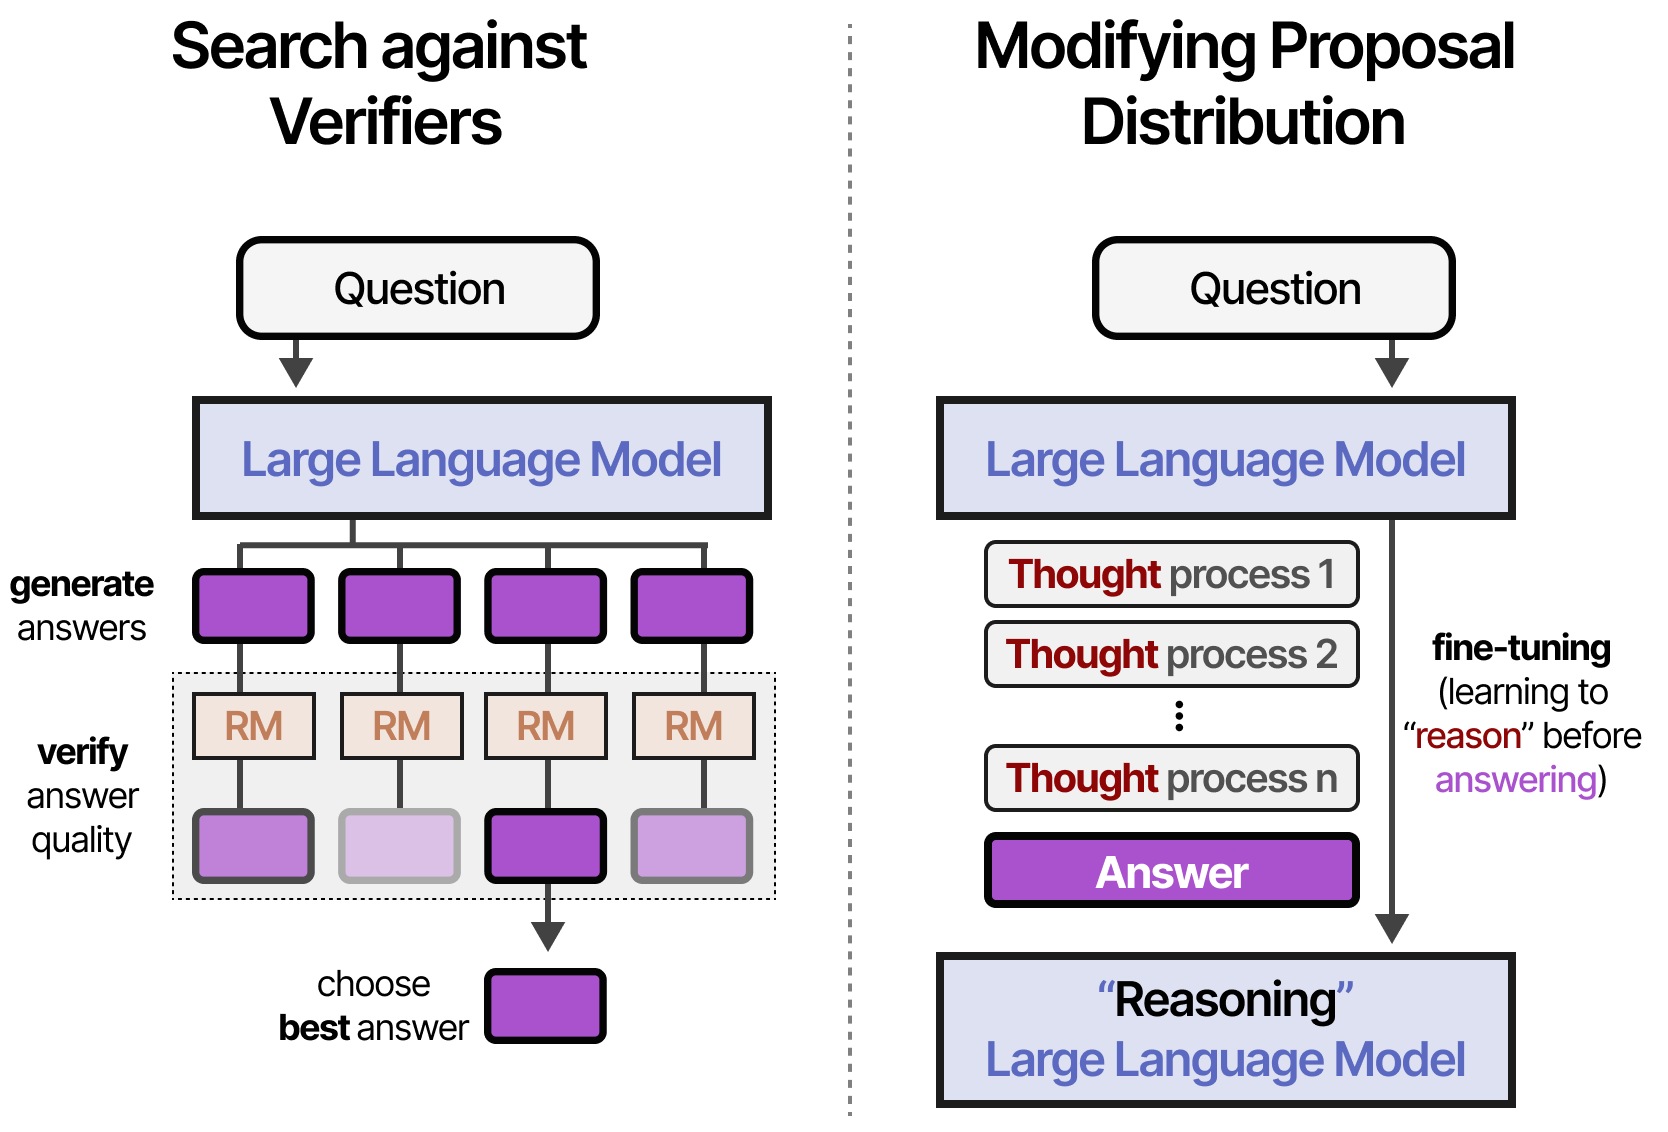
\includegraphics[width=0.4\linewidth,keepaspectratio]{llm228}
		
        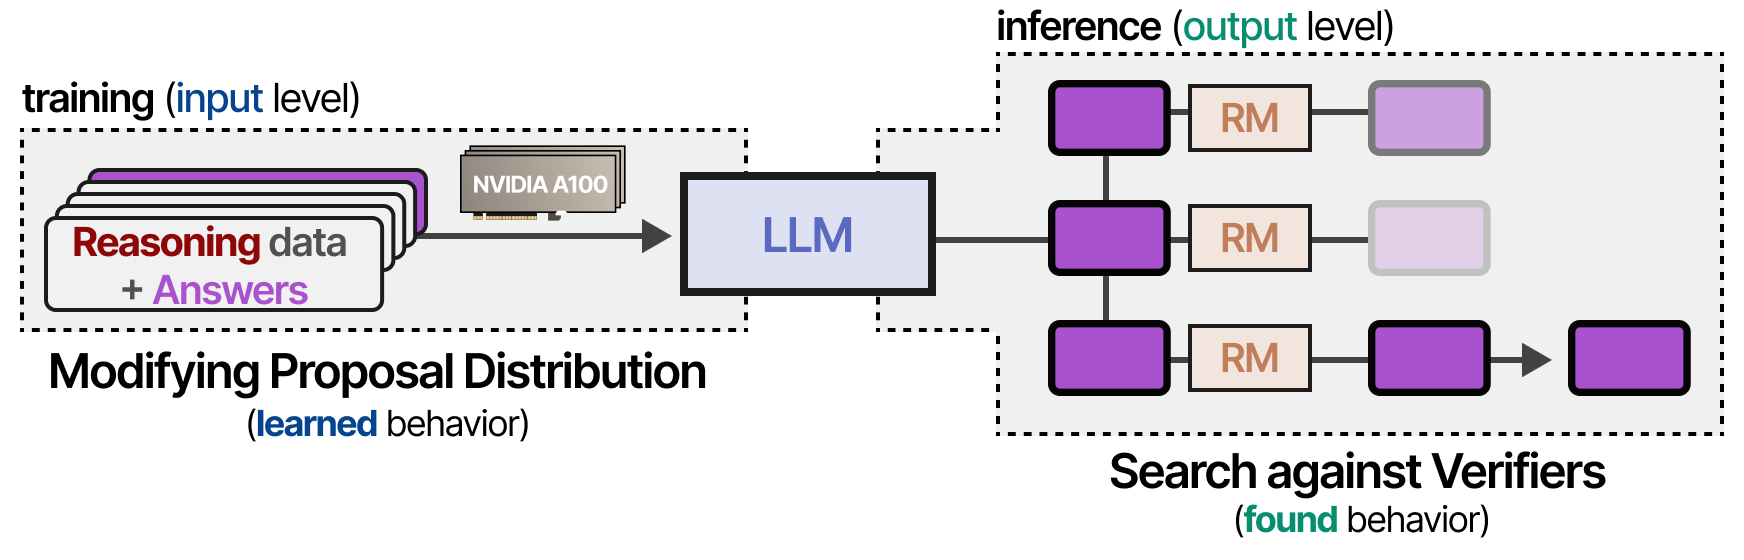
\includegraphics[width=0.4\linewidth,keepaspectratio]{llm229}
		
		{\tiny (Ref: Understanding How LLM learns to Reason and How to improve Reasoning - Vivedha Elango)}
        \end{center}		  
\end{frame}


%%%%%%%%%%%%%%%%%%%%%%%%%%%%%%%%%%%%%%%%%%%%%%%%%%%%%%%%%%%
\begin{frame}[fragile]\frametitle{Introduction to Search Against Verifiers}
      \begin{itemize}
        \item `Search against verifiers' is another category of test time compute different from plain prompting
        \item Verification means generating multiple answers and selecting the best one
        \item Instead of one answer, reasoning models provide multiple answers (A1, A2, A3, A4)
        \item A verification layer evaluates and selects the best answer from all generated responses
        \item This approach increases computational resources during inference time
        \item Similar to selecting the best quality crop from multiple samples in a field
        \item Increases probability of getting the optimal answer through sampling and verification
      \end{itemize}
	  
	  \begin{columns}
    \begin{column}[T]{0.5\linewidth}
        \begin{center}
        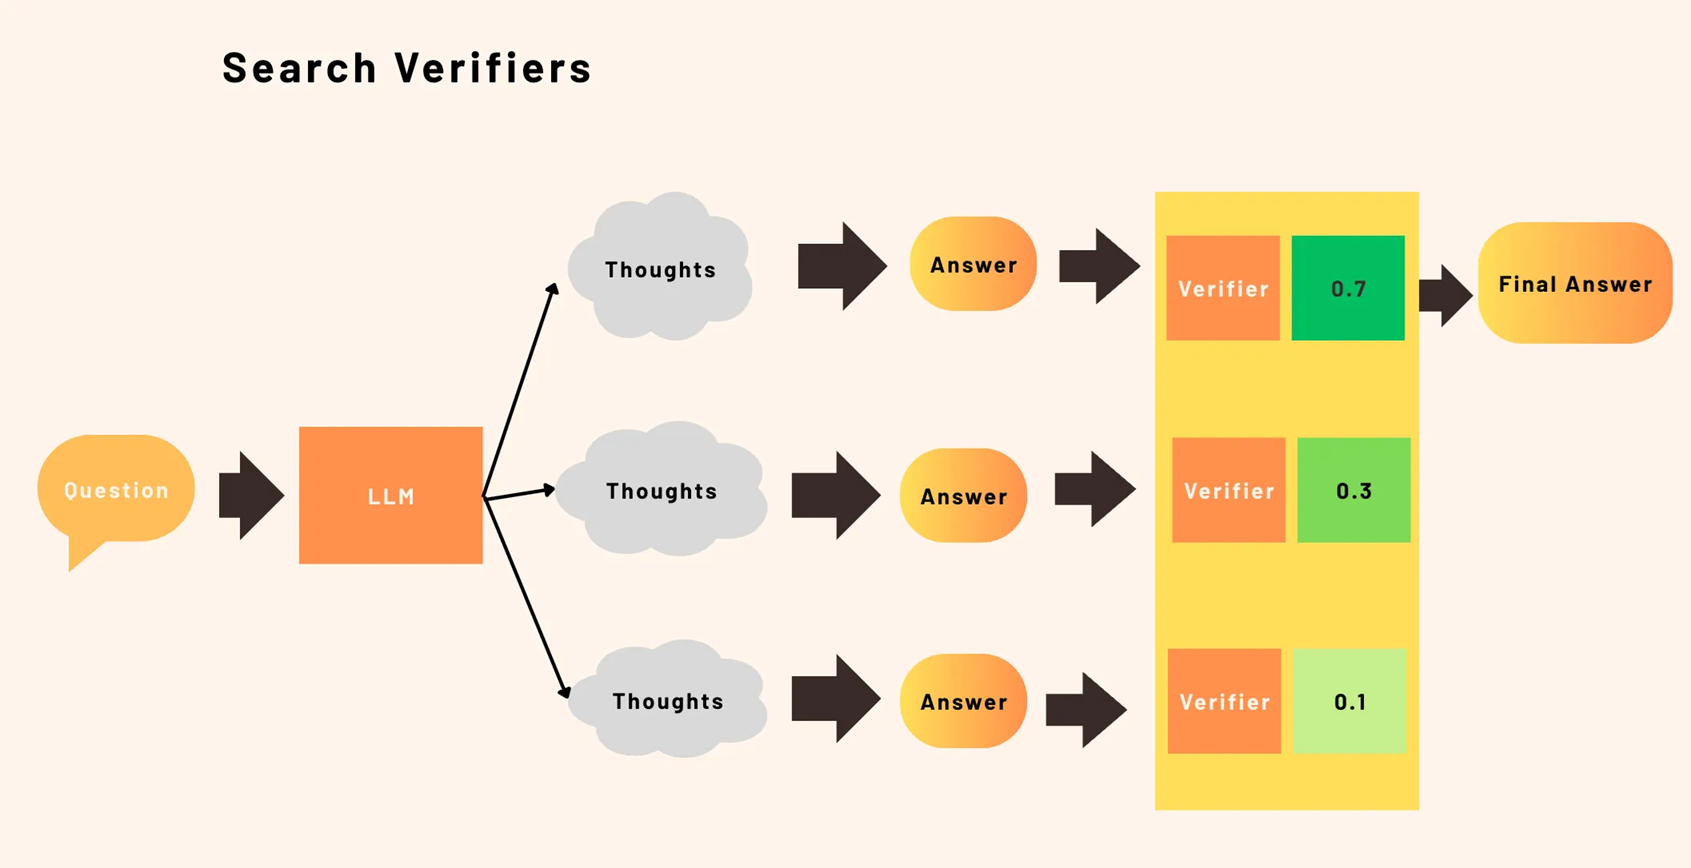
\includegraphics[width=\linewidth,keepaspectratio]{llm221}
		
		{\tiny (Ref: Understanding How LLM learns to Reason and How to improve Reasoning - Vivedha Elango)}
        \end{center}	

    \end{column}
    \begin{column}[T]{0.5\linewidth}
		\begin{center}
        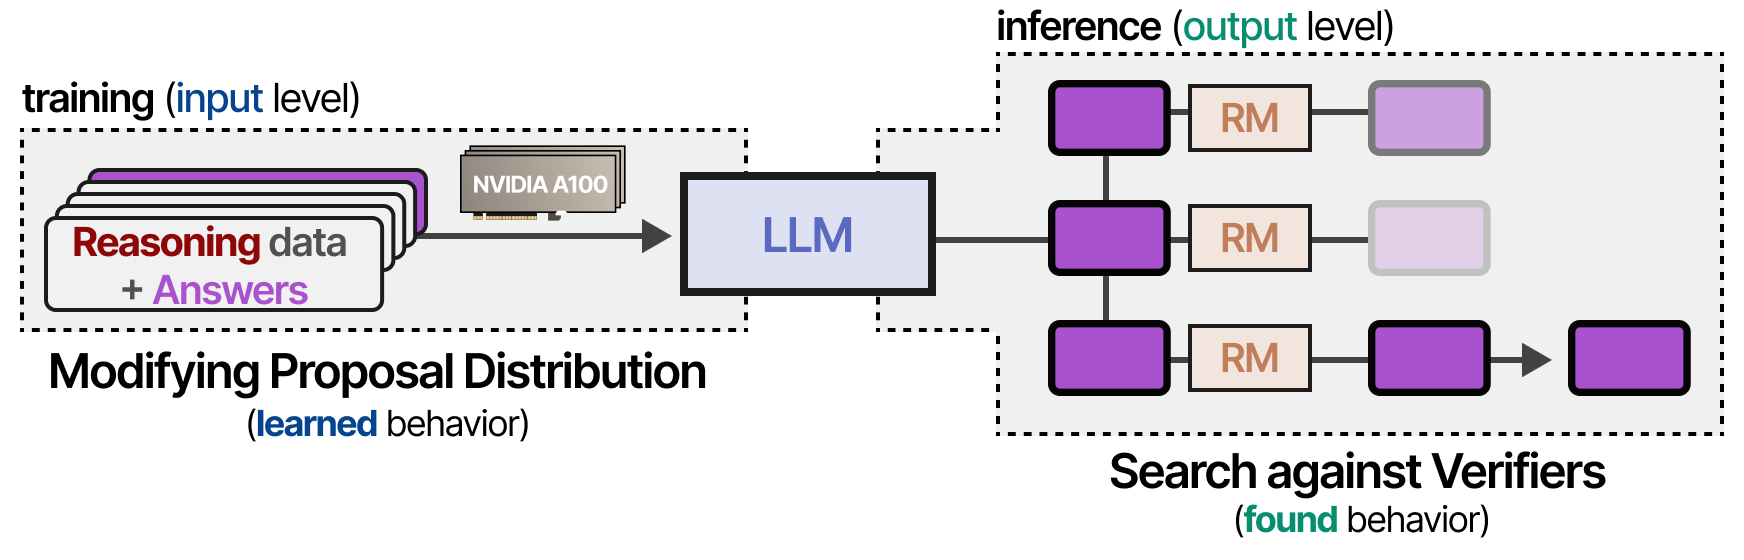
\includegraphics[width=\linewidth,keepaspectratio]{llm229}
		
		{\tiny (Ref: A Visual Guide to Reasoning LLMs - Maarten Grootendorst)}
		
		\end{center}
    \end{column}
  \end{columns}
  
	  
\end{frame}

%%%%%%%%%%%%%%%%%%%%%%%%%%%%%%%%%%%%%%%%%%%%%%%%%%%%%%%%%%%
\begin{frame}[fragile]\frametitle{Inference Time Compute Scaling}
      \begin{itemize}
        \item Verification layers increase computational resources used during LLM inference
        \item Standard LLM pipeline: pre-training → fine-tuning → inference
        \item Without verification: direct inference response
        \item With verification: extended inference time due to sampling and selection
        \item Process involves sampling different answers and selecting the best one
        \item Fits under inference time compute scaling because it increases response time
        \item Verification can be performed by humans or specialized models
      \end{itemize}
	  
	  \begin{columns}
    \begin{column}[T]{0.5\linewidth}
 	  
        \begin{center}
        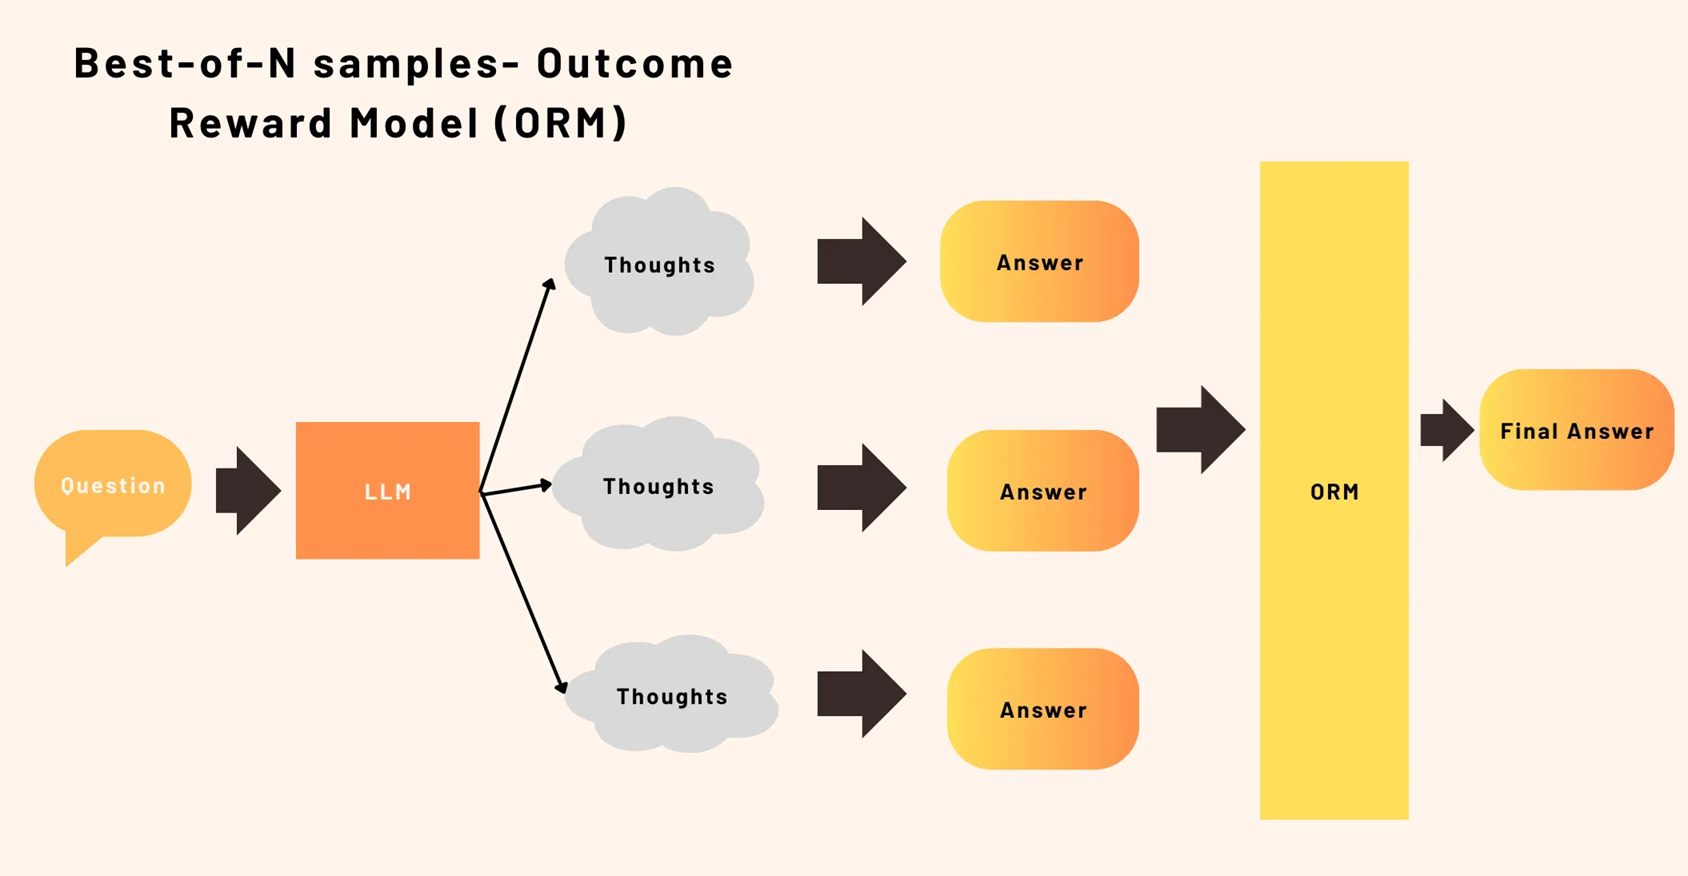
\includegraphics[width=0.5\linewidth,keepaspectratio]{llm222}
		
		{\tiny (Ref: Understanding How LLM learns to Reason and How to improve Reasoning - Vivedha Elango)}
        \end{center}	

    \end{column}
    \begin{column}[T]{0.5\linewidth}
		\begin{center}
        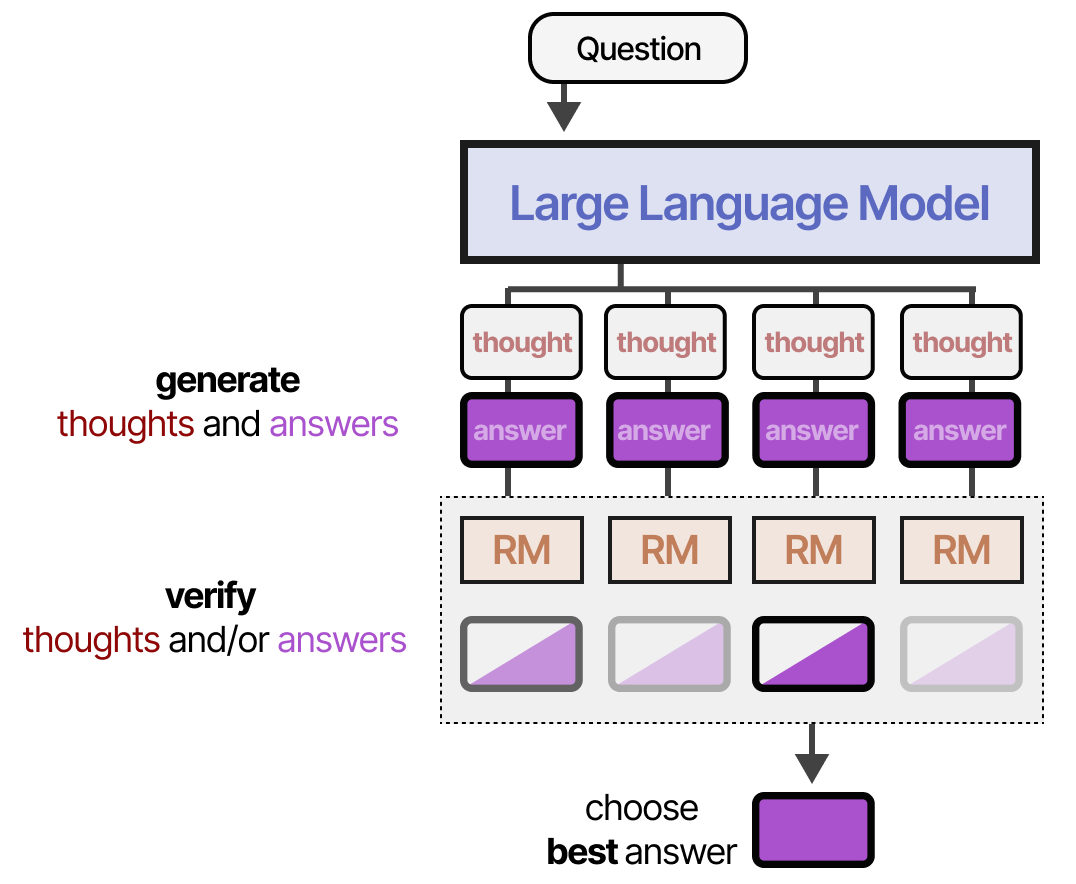
\includegraphics[width=0.7\linewidth,keepaspectratio]{llm233}
		
		{\tiny (Ref: A Visual Guide to Reasoning LLMs - Maarten Grootendorst)}
		
		\end{center}
    \end{column}
  \end{columns}	  
	  
\end{frame}

%%%%%%%%%%%%%%%%%%%%%%%%%%%%%%%%%%%%%%%%%%%%%%%%%%%%%%%%%%%
\begin{frame}[fragile]\frametitle{Reward Models for Verification}
      \begin{itemize}
        \item Models that perform verification are called reward models
        \item Example: reward-model-deberta-v3-large-v2 on Hugging Face
        \item Trained to predict which generated answer is better judged by humans
        \item Used for model evaluation, reward scoring in RLHF, and toxic response detection
        \item Training data generated by humans to mimic human verification ability
        \item Best answers are rewarded with maximum scores, poor answers get lower scores
        \item Essentially replacing human verifiers with trained models
      \end{itemize}
	  
        \begin{center}
        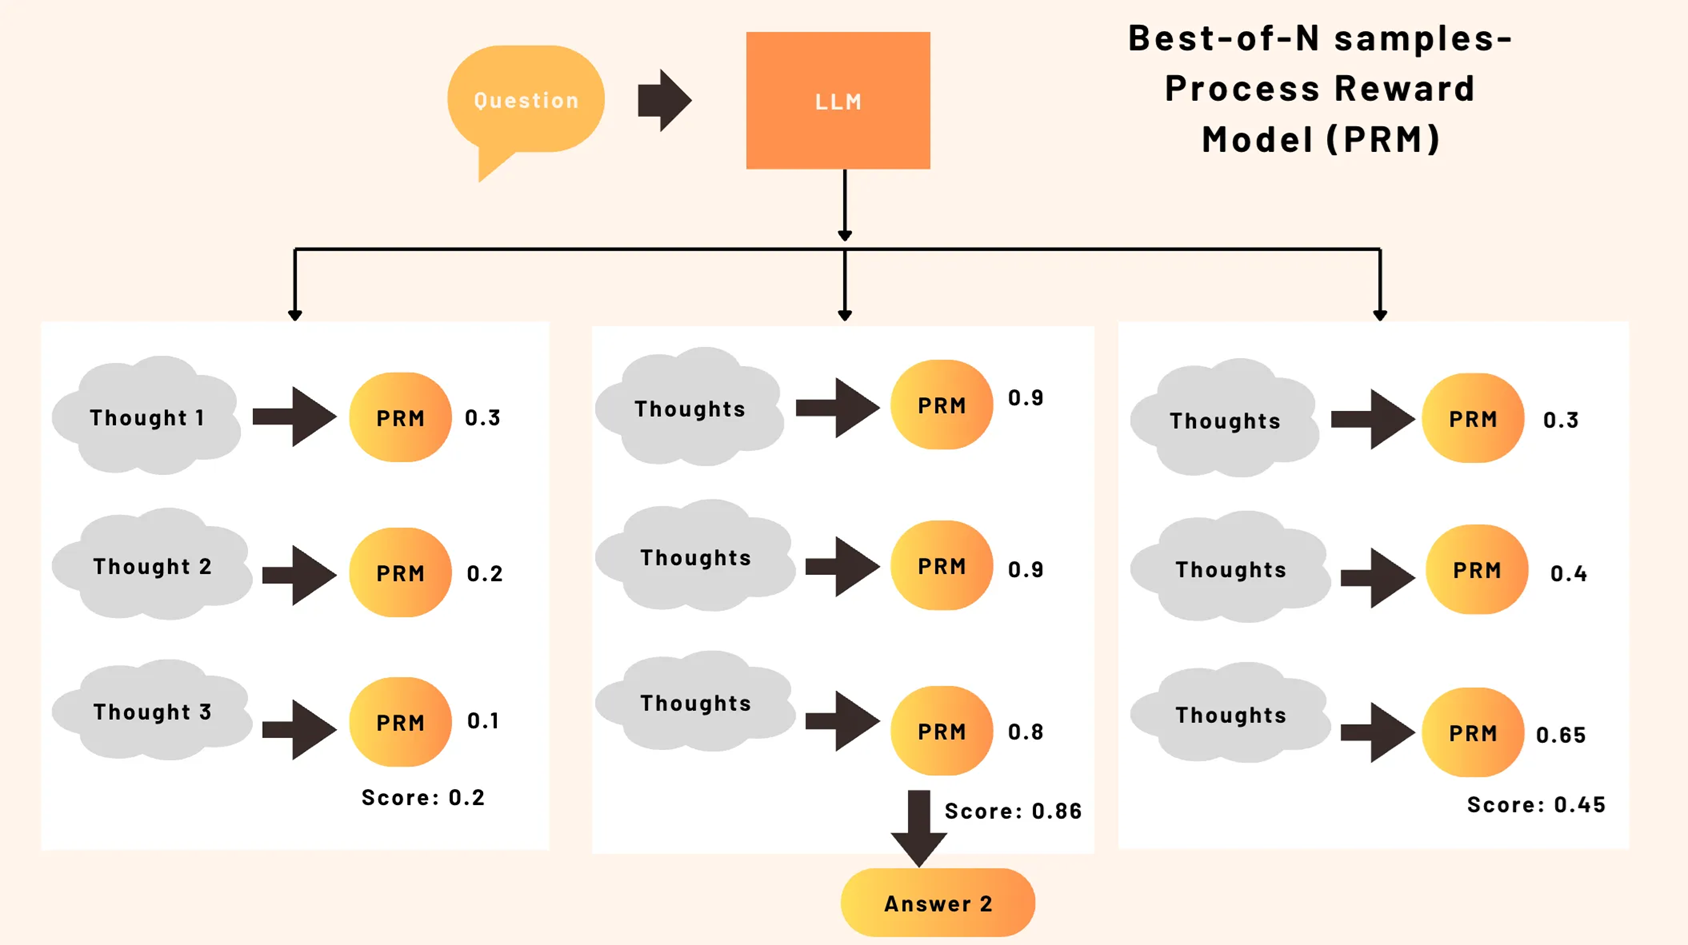
\includegraphics[width=0.5\linewidth,keepaspectratio]{llm223}
		
		{\tiny (Ref: Understanding How LLM learns to Reason and How to improve Reasoning - Vivedha Elango)}
        \end{center}		  
\end{frame}

%%%%%%%%%%%%%%%%%%%%%%%%%%%%%%%%%%%%%%%%%%%%%%%%%%%%%%%%%%%
\begin{frame}[fragile]\frametitle{Types of Reward Models}
      \begin{itemize}
        \item Two main categories: Outcome Reward Models (OM) and Process Reward Models (PRM)
        \item Outcome Reward Models: Only evaluate the final answer, ignore thought process
        \item OM doesn't care about reasoning steps, only scores the final outcome
        \item Process Reward Models: Evaluate individual reasoning steps leading to the answer
        \item PRM scores each thought in the chain of reasoning separately
        \item PRM assumes correct reasoning steps lead to correct final answers
        \item Process reward models are more popular and effective in practice
      \end{itemize}
	  
	  
\begin{columns}
    \begin{column}[T]{0.5\linewidth}
		\begin{center}
        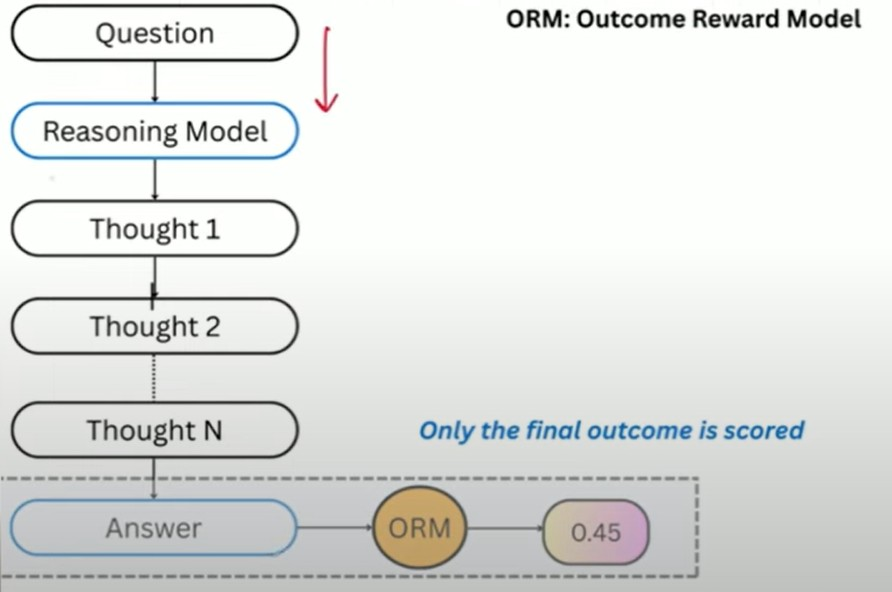
\includegraphics[width=0.7\linewidth,keepaspectratio]{llm224}
		\end{center}

    \end{column}
    \begin{column}[T]{0.5\linewidth}
		\begin{center}
        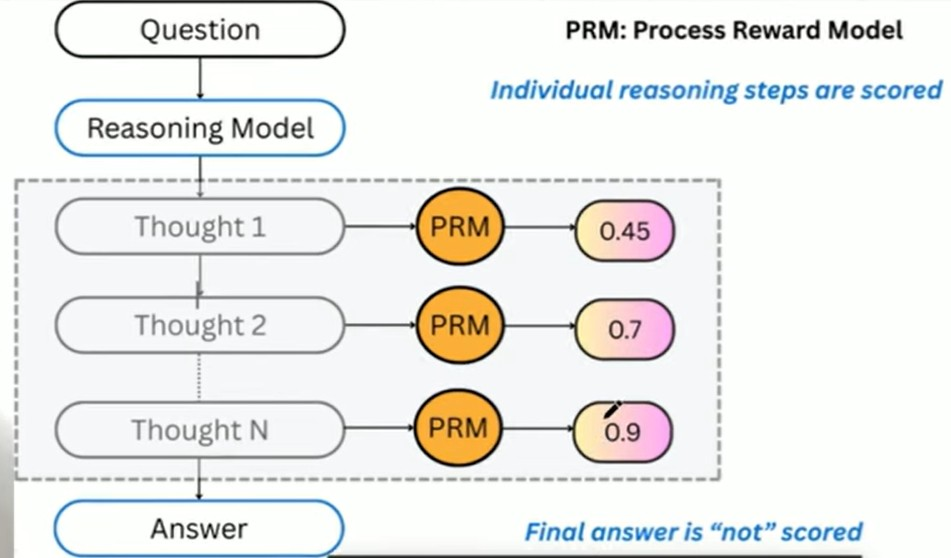
\includegraphics[width=0.8\linewidth,keepaspectratio]{llm225}
		\end{center}
    \end{column}
  \end{columns}
		
		
		{\tiny (Ref:  Reasoning LLMs from Scratch Series - Vizuara)}
  
\end{frame}


%%%%%%%%%%%%%%%%%%%%%%%%%%%%%%%%%%%%%%%%%%%%%%%%%%%%%%%%%%%
\begin{frame}[fragile]\frametitle{Types of Reward Models}
  
	  
\begin{columns}
    \begin{column}[T]{0.5\linewidth}
		\begin{center}
        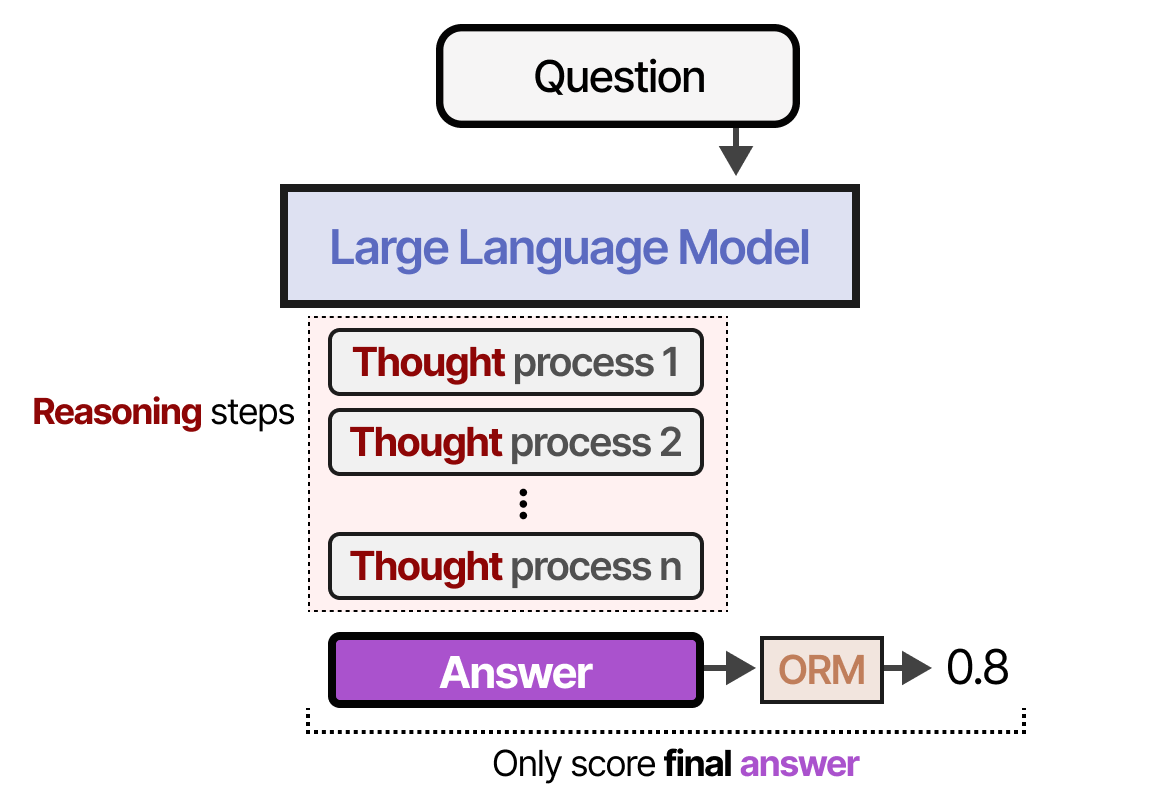
\includegraphics[width=0.7\linewidth,keepaspectratio]{llm230}
		\end{center}

    \end{column}
    \begin{column}[T]{0.5\linewidth}
		\begin{center}
        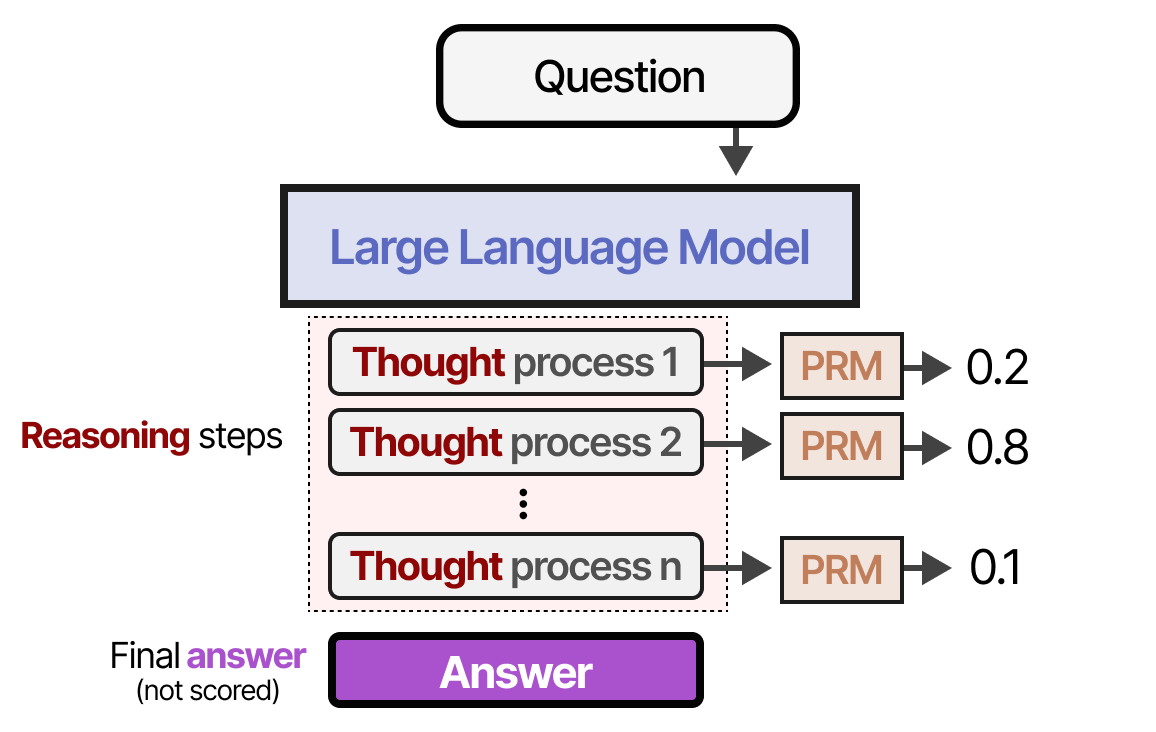
\includegraphics[width=0.8\linewidth,keepaspectratio]{llm231}
		\end{center}
    \end{column}
  \end{columns}
		
        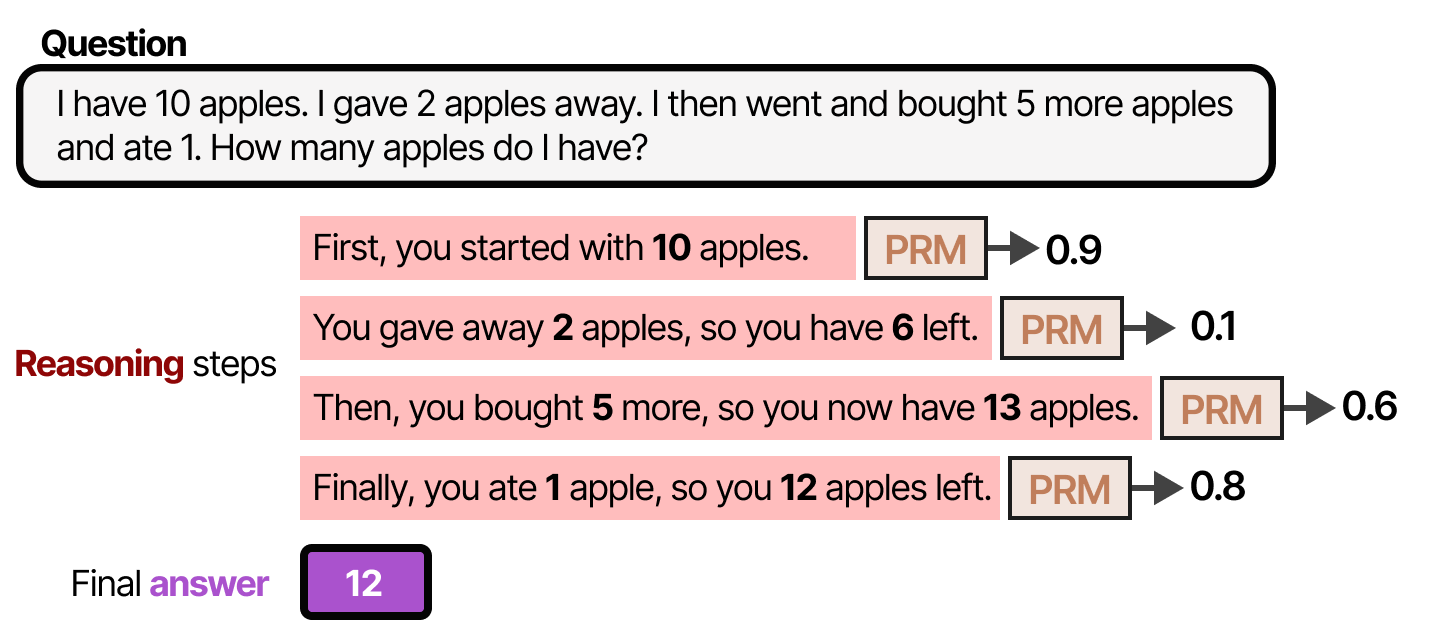
\includegraphics[width=0.8\linewidth,keepaspectratio]{llm232}
		
		
		{\tiny (Ref: A Visual Guide to Reasoning LLMs - Maarten Grootendorst)}
  
\end{frame}

%%%%%%%%%%%%%%%%%%%%%%%%%%%%%%%%%%%%%%%%%%%%%%%%%%%%%%%%%%%
\begin{frame}[fragile]\frametitle{Process Reward Model Example}
      \begin{itemize}
        \item Example: "Roger has 5 tennis balls, buys 2 cans with 3 balls each"
        \item Step 1: "Roger started with 5 balls" - Correct, gets higher score
        \item Step 2: "Two cans of 3 balls each is 5 balls" - Incorrect (should be 6), lower score
        \item Step 3: "Total is 5 + 6 = 11" - Correct calculation, gets higher score
        \item Wrong reasoning receives lower rewards, correct reasoning gets higher rewards
        \item Individual reasoning steps are evaluated rather than just the final answer
        \item Emphasizes the importance of correct chain of thought reasoning
      \end{itemize}
	  
        \begin{center}
        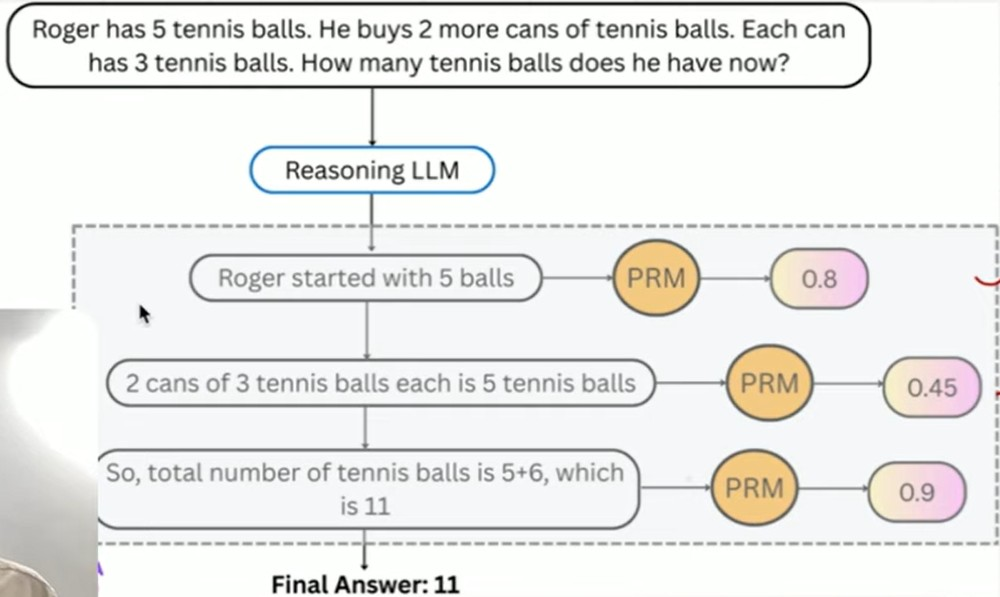
\includegraphics[width=0.5\linewidth,keepaspectratio]{llm226}
		
		{\tiny (Ref:  Reasoning LLMs from Scratch Series - Vizuara)}
        \end{center}		  
\end{frame}

%%%%%%%%%%%%%%%%%%%%%%%%%%%%%%%%%%%%%%%%%%%%%%%%%%%%%%%%%%%
\begin{frame}[fragile]\frametitle{Advantages of Verifiers}
      \begin{itemize}
        \item No need to fine-tune or retrain the base LLM for reasoning tasks
        \item Reasoning models like O1, DeepSeek likely use verification layers
        \item Process reward models evaluate answers before providing final response
        \item Ensures the answer with the best possible reasoning path is selected
        \item Maintains the original LLM while adding verification capability
        \item Cost-effective approach compared to retraining entire models
        \item Allows for modular improvement of reasoning capabilities
      \end{itemize}
\end{frame}

%%%%%%%%%%%%%%%%%%%%%%%%%%%%%%%%%%%%%%%%%%%%%%%%%%%%%%%%%%%
\begin{frame}[fragile]\frametitle{Types of Verifiers: Majority Voting}
      \begin{itemize}
        \item Most intuitive verification method, also called self-consistency
        \item Generate multiple answer samples (e.g., 10 answers) from the LLM
        \item Select the answer that appears the maximum number of times
        \item Example: Question about prime numbers finite - 2 "yes", 4 "no" → choose "no"
        \item No actual verifier model used, just statistical majority selection
        \item Main drawback: Answer can be wrong as there's no quality evaluation
        \item Simple but potentially unreliable verification approach
      \end{itemize}
	  
        % \begin{center}
        % 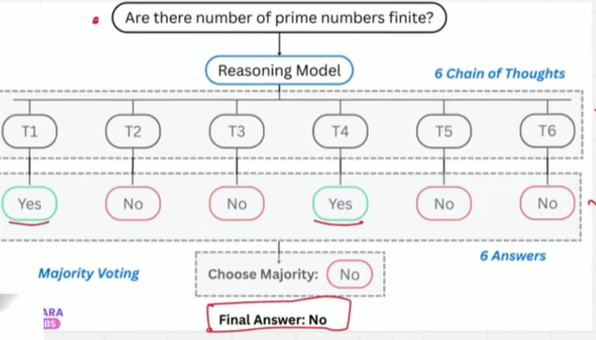
\includegraphics[width=0.5\linewidth,keepaspectratio]{llm227}
		
		% {\tiny (Ref:  Reasoning LLMs from Scratch Series - Vizuara)}
        % \end{center}	

		\begin{center}
        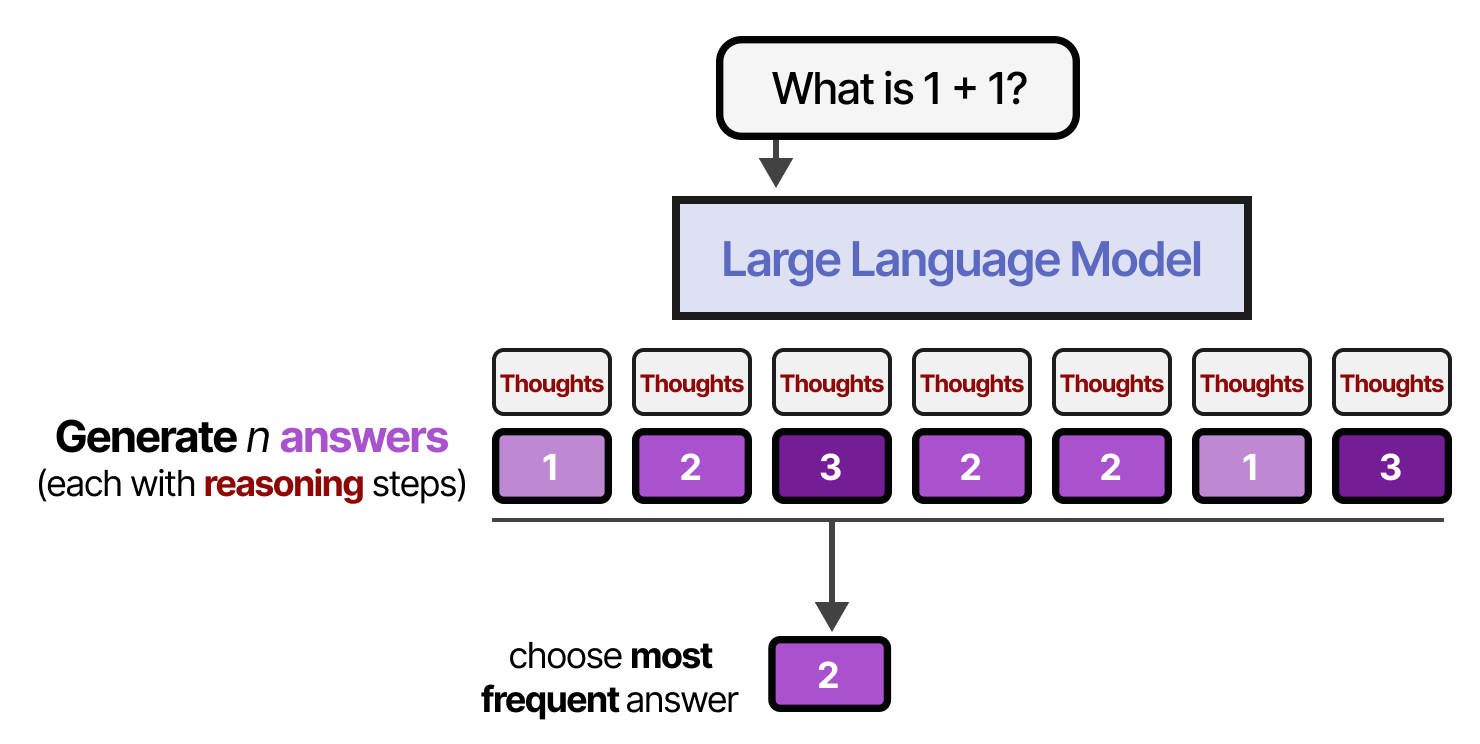
\includegraphics[width=0.7\linewidth,keepaspectratio]{llm234}
		
		{\tiny (Ref: A Visual Guide to Reasoning LLMs - Maarten Grootendorst)}
		
		\end{center}		
\end{frame}

%%%%%%%%%%%%%%%%%%%%%%%%%%%%%%%%%%%%%%%%%%%%%%%%%%%%%%%%%%%
\begin{frame}[fragile]\frametitle{Types of Verifiers: Best of N Samples}
      \begin{itemize}
        \item Generate N samples from the LLM, then apply verification layer
        \item Choose answer with maximum verifier score, not just majority
        \item Can use either Outcome Reward Model (OM) or Process Reward Model (PRM)
        \item OM example: Score final answers (91, 95, 82, 76, 14), select highest scored
        \item PRM example: Score reasoning chains, calculate weighted averages
        \item Select answer with best average reasoning score in PRM approach
        \item More reliable than majority voting as it evaluates answer quality
      \end{itemize}
	  
	  
        % \begin{center}
        % 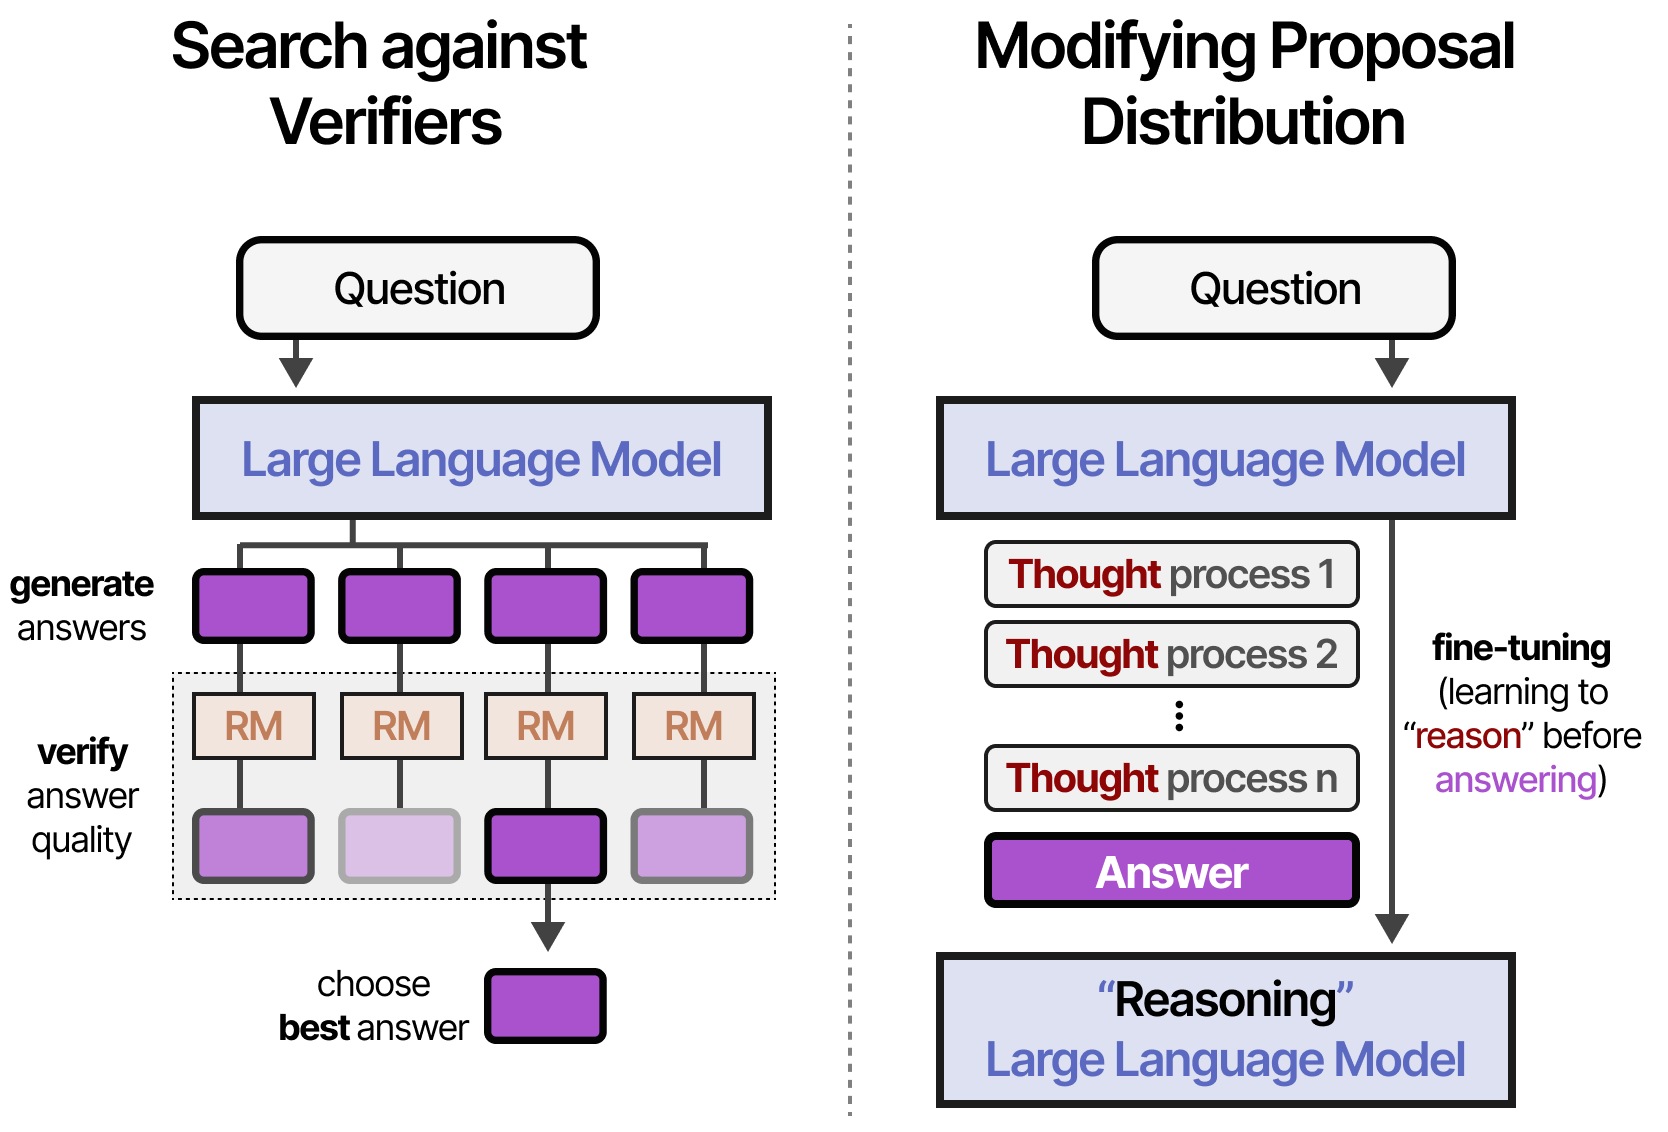
\includegraphics[width=0.5\linewidth,keepaspectratio]{llm228}
		
		% {\tiny (Ref:  Reasoning LLMs from Scratch Series - Vizuara)}
        % \end{center}		
\end{frame}

%%%%%%%%%%%%%%%%%%%%%%%%%%%%%%%%%%%%%%%%%%%%%%%%%%%%%%%%%%%
\begin{frame}[fragile]\frametitle{Types of Verifiers: Best of N Samples}
	  
	
		\begin{center}
        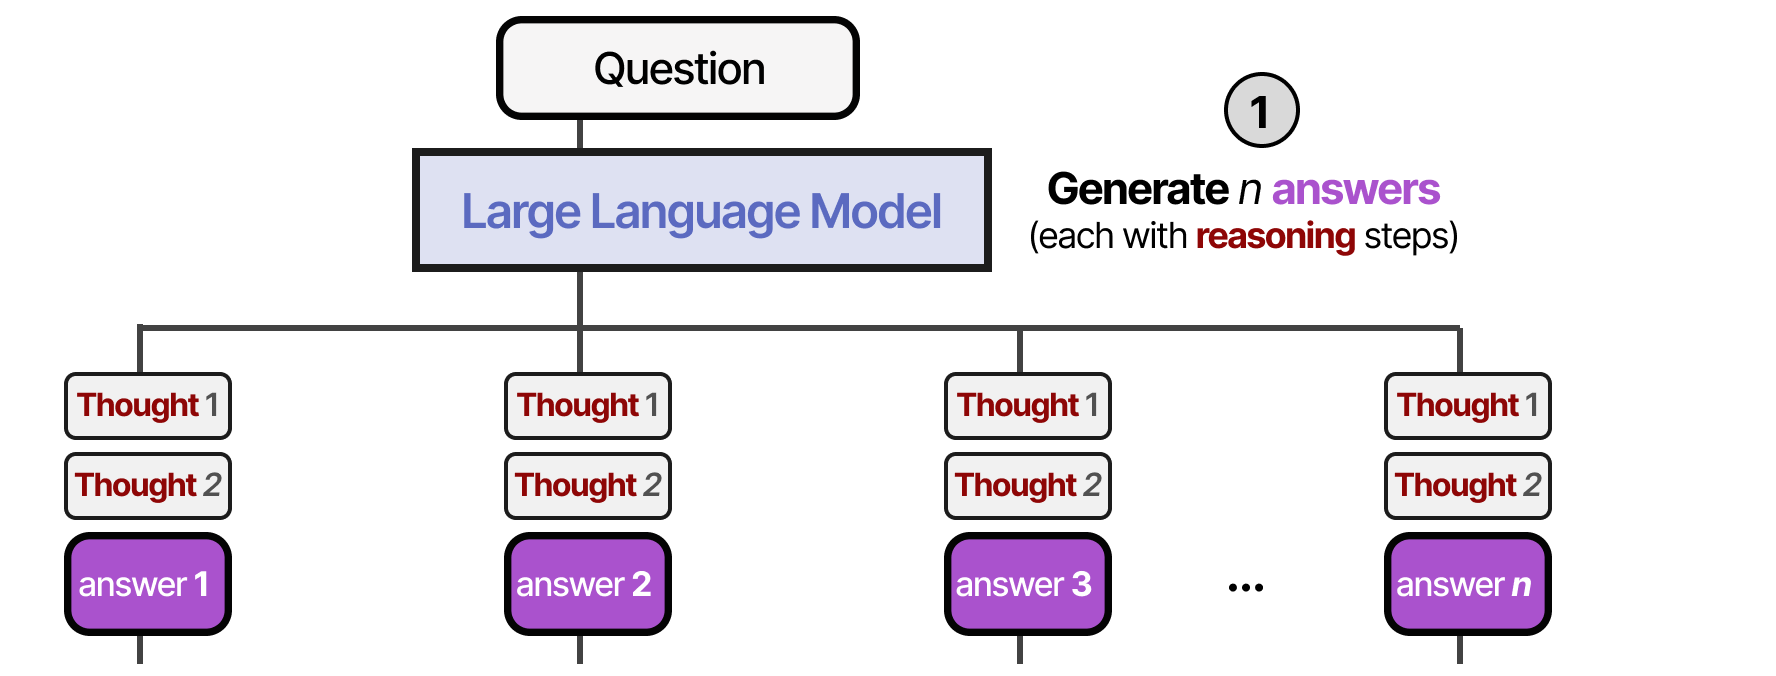
\includegraphics[width=\linewidth,keepaspectratio]{llm235}
		
	
		{\tiny (Ref: A Visual Guide to Reasoning LLMs - Maarten Grootendorst)}
		
		\end{center}			
\end{frame}

%%%%%%%%%%%%%%%%%%%%%%%%%%%%%%%%%%%%%%%%%%%%%%%%%%%%%%%%%%%
\begin{frame}[fragile]\frametitle{Types of Verifiers: Best of N Samples}

		\begin{center}
		
        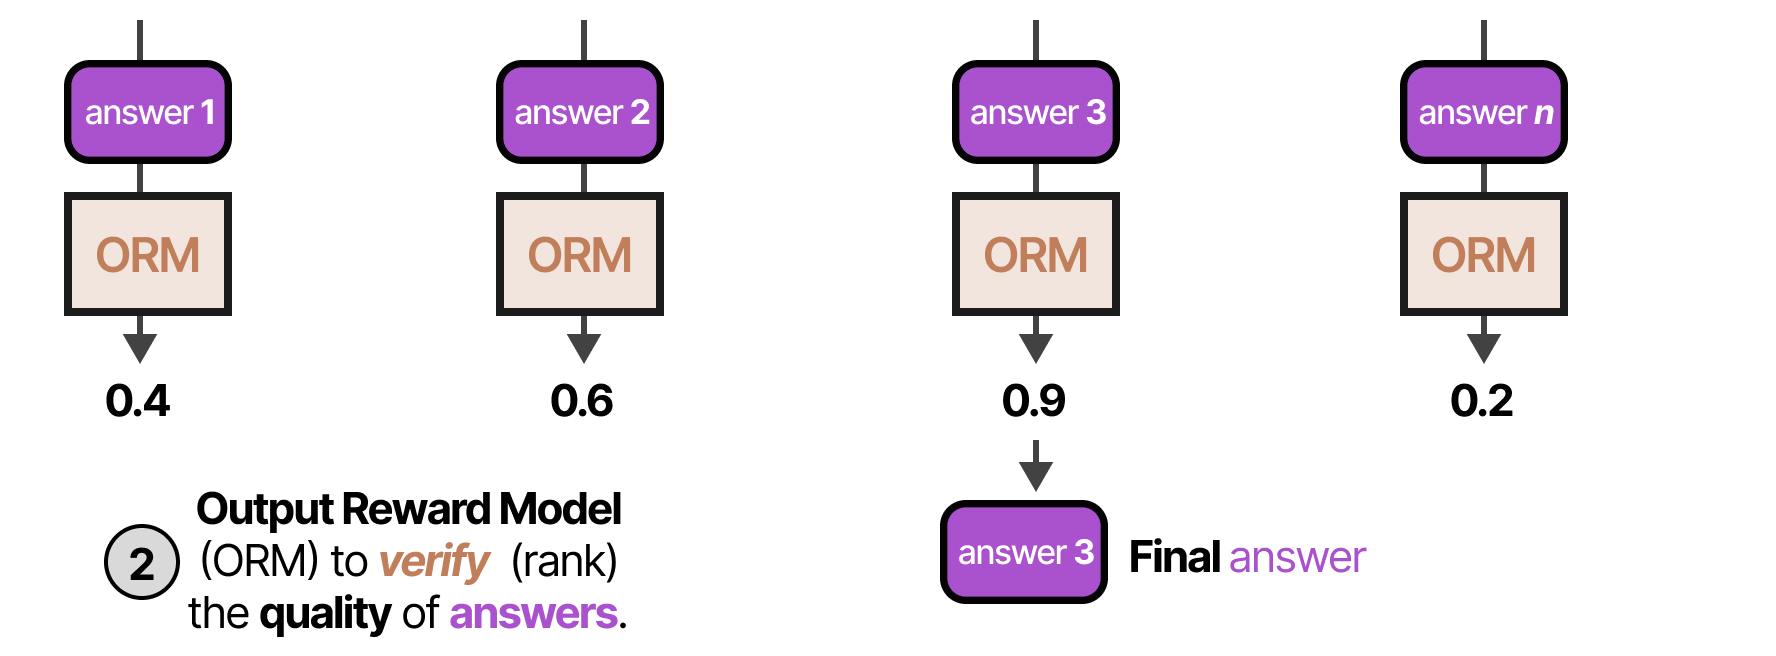
\includegraphics[width=\linewidth,keepaspectratio]{llm236}
		
		{\tiny (Ref: A Visual Guide to Reasoning LLMs - Maarten Grootendorst)}
		
		\end{center}			
\end{frame}


%%%%%%%%%%%%%%%%%%%%%%%%%%%%%%%%%%%%%%%%%%%%%%%%%%%%%%%%%%%
\begin{frame}[fragile]\frametitle{Types of Verifiers: Best of N Samples}
	
		\begin{center}
        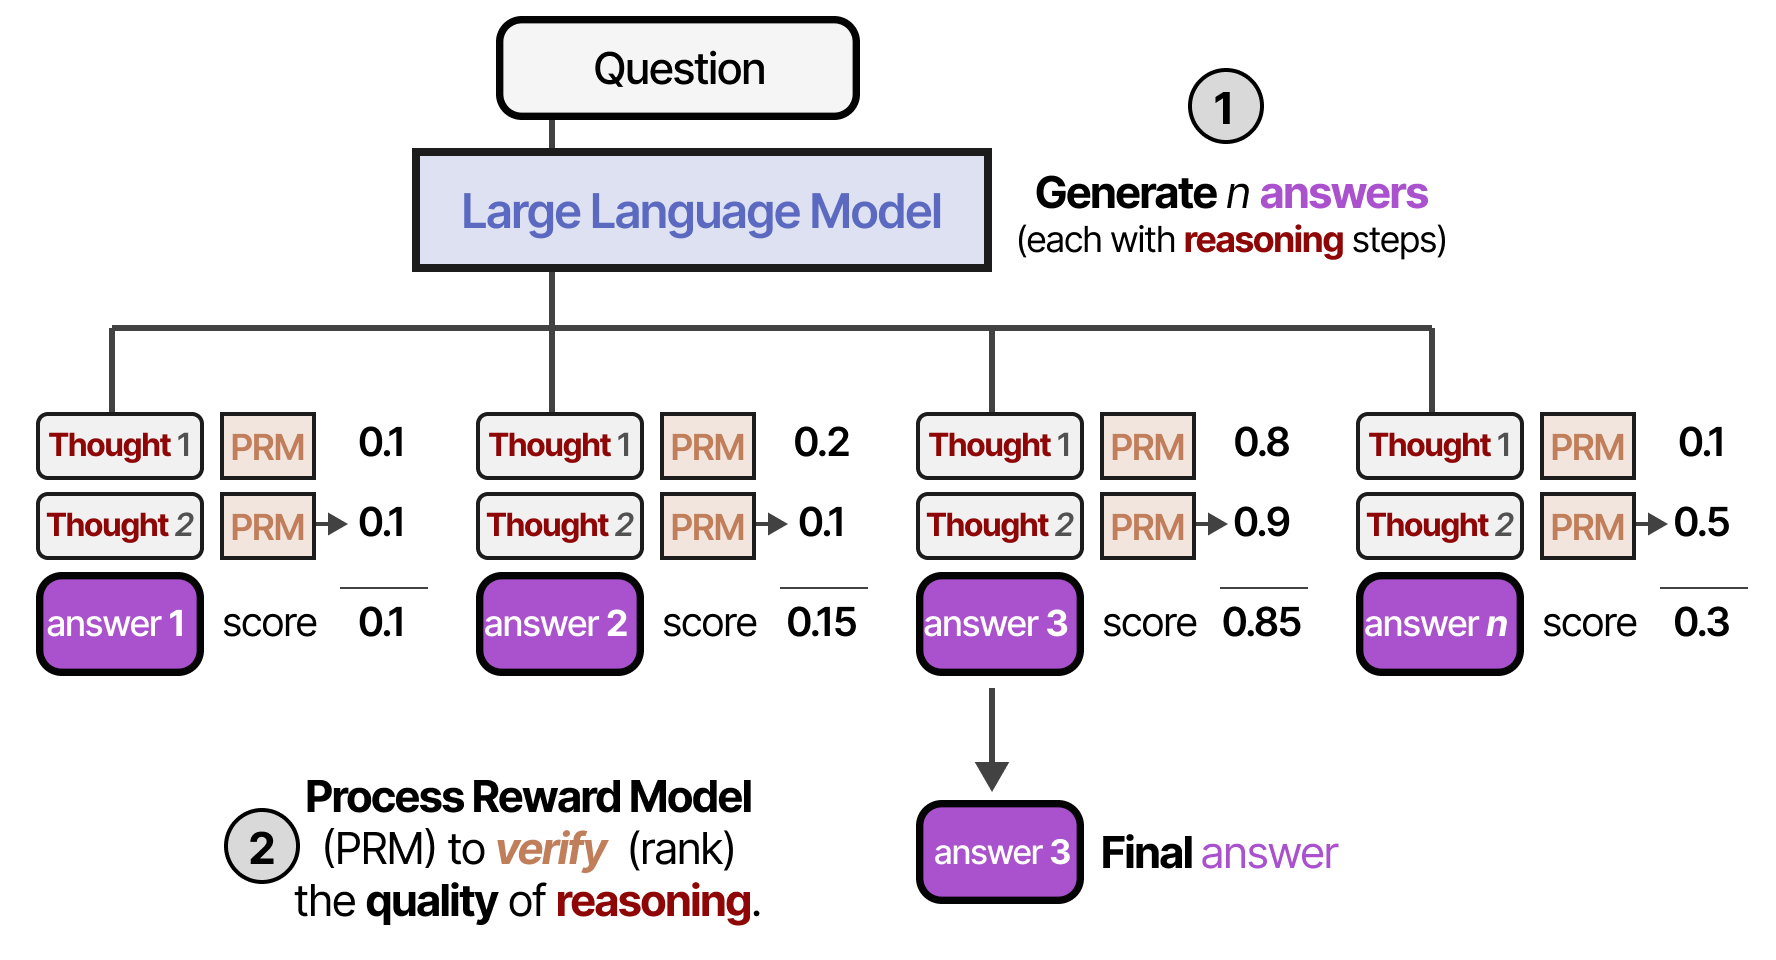
\includegraphics[width=\linewidth,keepaspectratio]{llm237}
		
	
		{\tiny (Ref: A Visual Guide to Reasoning LLMs - Maarten Grootendorst)}
		
		\end{center}			
\end{frame}


%%%%%%%%%%%%%%%%%%%%%%%%%%%%%%%%%%%%%%%%%%%%%%%%%%%%%%%%%%%
\begin{frame}[fragile]\frametitle{Types of Verifiers: Best of N Samples}
	
		\begin{center}
	
        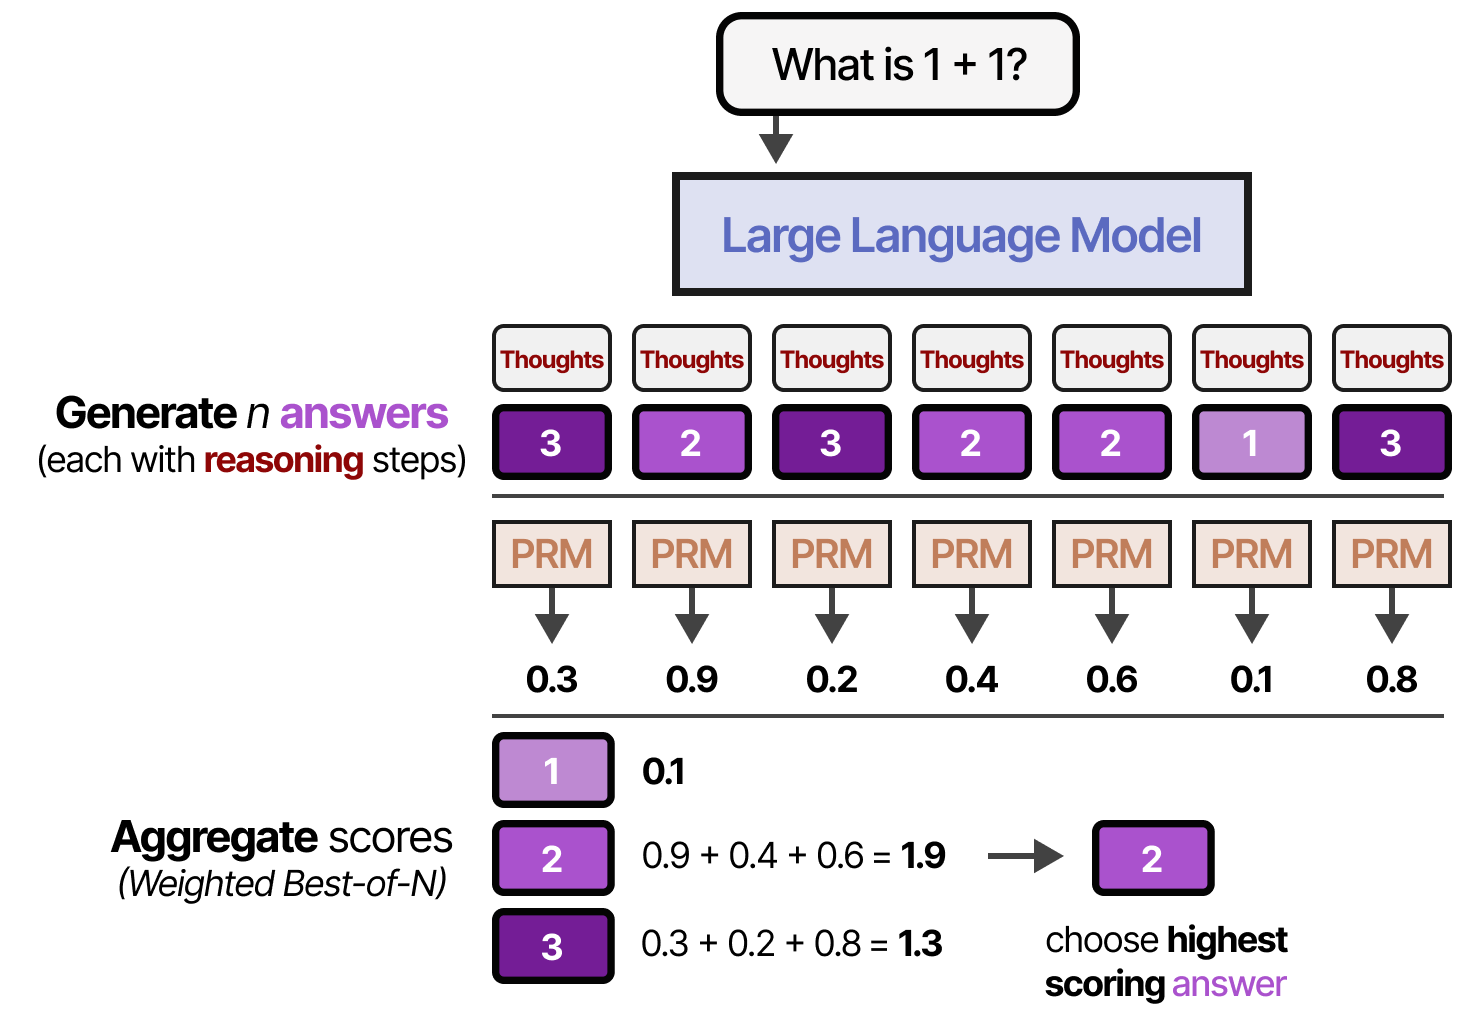
\includegraphics[width=0.8\linewidth,keepaspectratio]{llm238}
		
		{\tiny (Ref: A Visual Guide to Reasoning LLMs - Maarten Grootendorst)}
		
		\end{center}			
\end{frame}

%%%%%%%%%%%%%%%%%%%%%%%%%%%%%%%%%%%%%%%%%%%%%%%%%%%%%%%%%%%
\begin{frame}[fragile]\frametitle{Beam Search Algorithm Origins}
      \begin{itemize}
        \item Originally proposed in 1976 for speech recognition systems
        \item Paper: "The HARPY Speech Recognition System" - ancient algorithm (50 years old)
        \item Initially called "few best paths in parallel" search strategy
        \item Used extensively in speech recognition and translation tasks
        \item Not developed by modern LLM researchers, but adapted for AI reasoning
        \item Well-established algorithm with proven effectiveness across domains
        \item Now applied to construct effective verifiers for reasoning models
      \end{itemize}
\end{frame}

%%%%%%%%%%%%%%%%%%%%%%%%%%%%%%%%%%%%%%%%%%%%%%%%%%%%%%%%%%%
\begin{frame}[fragile]\frametitle{Beam Search Algorithm }
	
		\begin{center}
	
        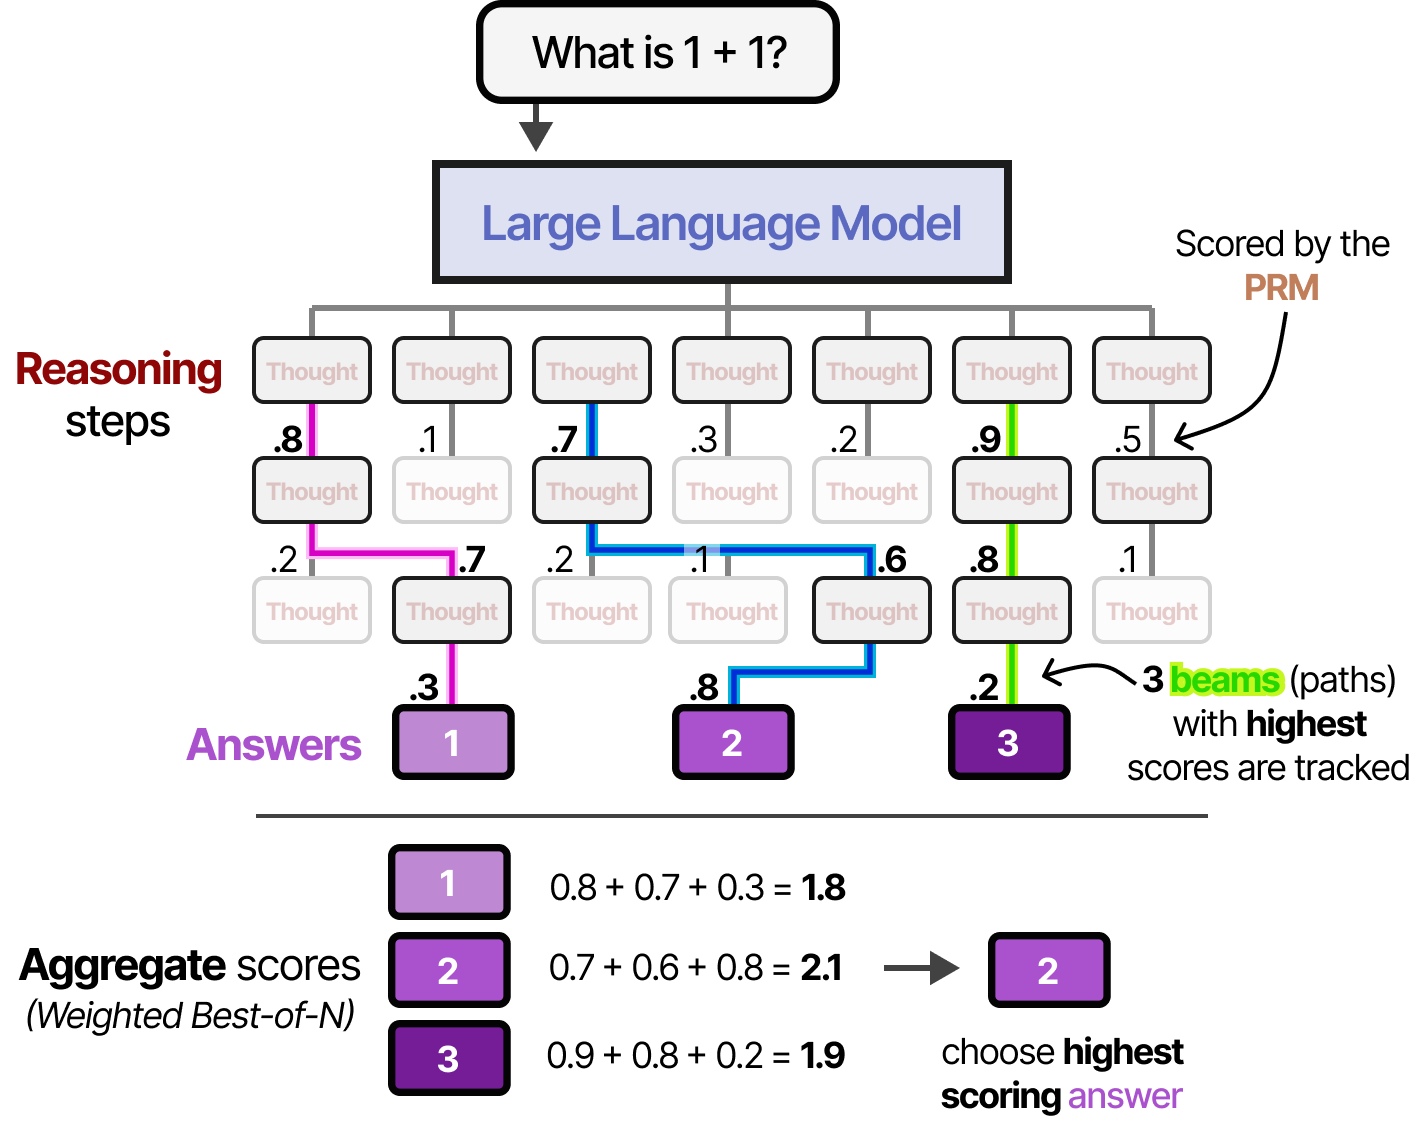
\includegraphics[width=0.8\linewidth,keepaspectratio]{llm239}
		
		{\tiny (Ref: A Visual Guide to Reasoning LLMs - Maarten Grootendorst)}
		
		\end{center}			
\end{frame}


%%%%%%%%%%%%%%%%%%%%%%%%%%%%%%%%%%%%%%%%%%%%%%%%%%%%%%%%%%%
\begin{frame}[fragile]\frametitle{Beam Search for Translation Example}
      \begin{itemize}
        \item Example: Translate Hindi sentence "mein dilhi jaa raha hun" to English
        \item Use text corpus of 50,000 words for translation vocabulary
        \item Step 1: Select 3 most probable first words (I, Delhi, zoo)
        \item Step 2: Evaluate 150,000 combinations, select best 3 two-word combinations
        \item Step 3: Continue process, eliminating less probable paths
        \item Beam width = 3 (number of candidates kept at each step)
        \item Progressive elimination leads to optimal translation path
      \end{itemize}
	  
		\begin{center}
	
        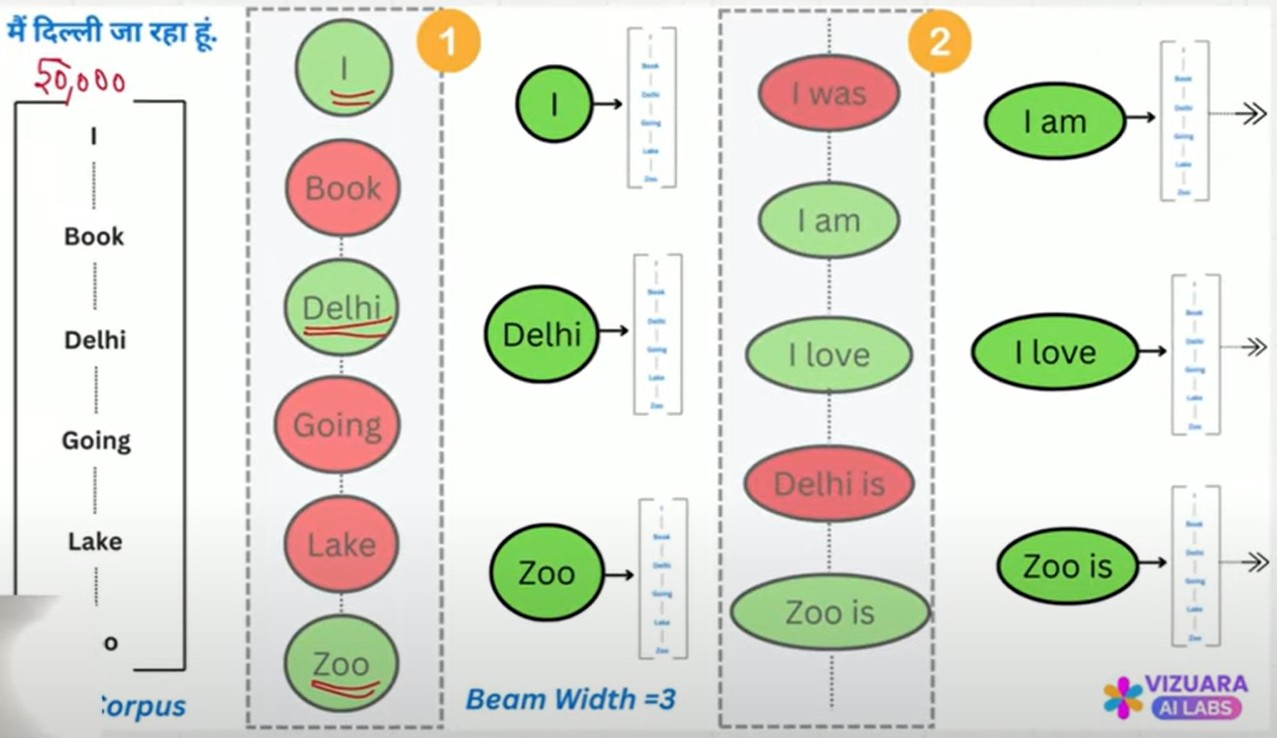
\includegraphics[width=0.5\linewidth,keepaspectratio]{llm240}
		
		{\tiny (Ref:  Reasoning LLMs from Scratch Series - Vizuara)}
		
		\end{center}		  
\end{frame}

%%%%%%%%%%%%%%%%%%%%%%%%%%%%%%%%%%%%%%%%%%%%%%%%%%%%%%%%%%%
\begin{frame}[fragile]\frametitle{Beam Search Parameters}
      \begin{itemize}
        \item Two key parameters: Number of beams and Beam width
        \item Number of beams: Total paths explored simultaneously (e.g., 4)
        \item Beam width: Number of best candidates kept at each step (e.g., 2)
        \item Generate multiple thoughts, select best ones based on scores
        \item Purple background represents verifier scoring each thought
        \item Process repeats: generate → score → select → branch → repeat
        \item Final selection provides optimal reasoning path to answer
      \end{itemize}
	  
		\begin{center}
	
        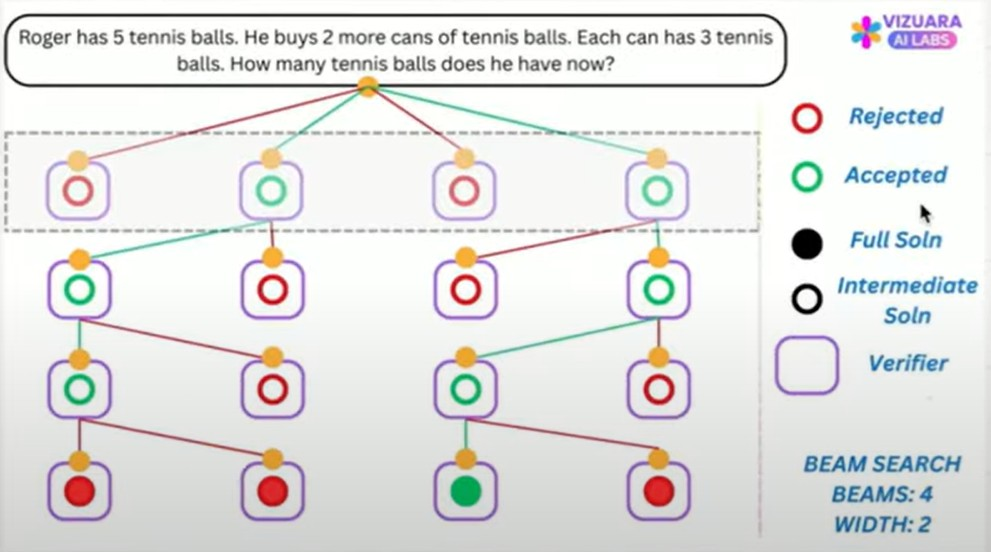
\includegraphics[width=0.5\linewidth,keepaspectratio]{llm241}
		
		{\tiny (Ref:  Reasoning LLMs from Scratch Series - Vizuara)}
		
		\end{center}			  
\end{frame}

%%%%%%%%%%%%%%%%%%%%%%%%%%%%%%%%%%%%%%%%%%%%%%%%%%%%%%%%%%%
\begin{frame}[fragile]\frametitle{Beam Search Implementation}
      \begin{itemize}
        \item Uses Process Reward Models for scoring reasoning steps
        \item Implementation requires reasoning model (e.g., Zephyr 7B) and reward model
        \item Google Colab notebook demonstrates practical beam search tree generation
        \item Visualization shows progressive selection through reasoning layers
        \item Temperature parameter affects answer variation and exploration
        \item Higher temperature (0.9) provides more diverse reasoning paths
        \item Code allows experimentation with different beam parameters
      \end{itemize}
\end{frame}

%%%%%%%%%%%%%%%%%%%%%%%%%%%%%%%%%%%%%%%%%%%%%%%%%%%%%%%%%%%
\begin{frame}[fragile]\frametitle{Two Categories of Improvement}
      \begin{itemize}
        \item Verifiers: Verification layer that grades generated answers
        \item Proposal Distribution Modification: Changing how answers are generated initially
        \item Chain of thought reasoning (few-shot and zero-shot) modifies proposal distribution
        \item Beam search, majority voting, best-of-N are verification techniques
        \item Both methods are viable for building reasoning models
        \item Can be combined: modify generation + add verification layer
        \item Represents comprehensive approach to inference time compute scaling
      \end{itemize}
\end{frame}